\chapter{Einleitung}

\section{Aufgabe/Motivation}

Ziel des Versuchs ist die Bestimmung der Faraday-Konstante $F$ mit zwei unterschiedlichen Verfahren und die qualitative Untersuchung einer Brennstoffzelle. Im ersten Verfahren wird die Elektrolyse einer Kupfersulfatlösung durchgeführt, wobei Kupferionen an der Kathode reduziert und abgeschieden werden. Die Massenänderung der Elektroden und die ermittelte transportierte Ladung ermöglichen die Berechnung der Faraday-Konstante über das erste Faraday’sche Gesetz. Im zweiten Verfahren erfolgt die elektrolytische Zersetzung von Wasser in einem Hoffmannschen Wasserzersetzungsapparat, wobei an der Kathode Wasserstoff und an der Anode Sauerstoff entstehen. Durch Messung der Gasvolumina und Berechnung der Stoffmengen kann erneut die Faraday-Konstante bestimmt werden.

Zusätzlich wird das Funktionsprinzip einer PEM-Brennstoffzelle betrachtet, die die umgekehrte Reaktion der Elektrolyse nutzt: Wasserstoff reagiert mit Sauerstoff unter kontrollierter Energieabgabe zu Wasser, wobei Elektronen über einen äußeren Stromkreis geleitet werden und elektrische Energie erzeugen.

\section{Physikalische Grundlage}

\cite{demtroeder17,skript25}

\subsection{Elektrolyse}

Elektrolyte sind Lösungen von Säuren, Hydroxiden, Salzen oder deren Schmelzen, die freie Ionen enthalten und dadurch elektrische Leiter darstellen. Im Gegensatz zu metallischen Leitern erfolgt der Ladungstransport hier über Ionen. Ionen entstehen aus neutralen Atomen oder Molekülen durch Abgabe oder Aufnahme von Elektronen oder durch Dissoziation. Positiv geladene Ionen (Kationen) wandern zur Kathode, negativ geladene Ionen (Anionen) zur Anode.  

Befindet sich ein Elektrolyt im Feld zweier Elektroden und es fließt Strom, wird der Elektrolyt in der Regel zersetzt. Dieser Vorgang wird als Elektrolyse bezeichnet.

\subsection{Faraday-Konstante}

Die Faraday-Konstante $F$ ist definiert als

\begin{equation}
F = e N_A = (9,648455 \pm 0,000027) \cdot 10^4 \,\mathrm{C\,mol^{-1}}
\label{eq:faraday}
\end{equation}

Sie gibt die Ladungsmenge an, die durch einen Elektrolyten fließt, wenn sich $1/z$ Mol eines $z$-wertigen Stoffes an der Elektrode abscheidet. Über das erste Faraday’sche Gesetz:

\begin{equation}
m = n \cdot M_\mathrm{Mol} = \frac{Q \cdot M_\mathrm{Mol}}{z \cdot F}
\label{eq:first_faraday}
\end{equation}

lässt sich die Faraday-Konstante berechnen, wobei $Q$ die transportierte Ladung, $z$ die Ionenwertigkeit, $n$ die abgeschiedene Stoffmenge und $M_\mathrm{Mol}$ die Molmasse des Stoffes ist.

\subsection{Bestimmung der Faraday-Konstante durch Massenmessung}
\label{sc:Massenmessung}

Für das erste Verfahren wird Kupfersulfat CuSO$_4$ in Wasser gelöst, das gemäß

\begin{equation}
\mathrm{CuSO_4 \rightleftharpoons Cu^{2+} + SO_4^{2-}}
\label{eq:cu_dissoziation}
\end{equation}

dissoziiert. Die Cu$^{2+}$-Ionen wandern zur Kathode, nehmen zwei Elektronen auf und werden zu Kupfer reduziert:

\begin{equation}
\mathrm{Cu^{2+} + 2e^- \rightarrow Cu}
\label{eq:cu_reduktion}
\end{equation}

Gleichzeitig wird an der Anode Kupfer oxidiert:

\begin{equation}
\mathrm{Cu \rightarrow Cu^{2+} + 2e^-}
\label{eq:cu_oxidation}
\end{equation}

Die Gesamtmenge an Kupfersulfat in der Lösung bleibt dabei unverändert. Die transportierte Ladung berechnet sich über

\begin{equation}
Q = I \cdot t
\label{eq:ladung}
\end{equation}

mit Stromstärke $I$ und Zeit $t$. Durch Wägung der Elektroden vor und nach der Elektrolyse kann die Faraday-Konstante $F$ ermittelt werden.

\subsection{Bestimmung der Faraday-Konstante durch Volumenmessung}
\label{sc:faraday_vol}

Im zweiten Verfahren wird die Zersetzung von Wasser im Hoffmannschen Wasserzersetzungsapparat untersucht. Dieser besteht aus zwei Schenkeln mit Platin-Elektroden und einem höhenverstellbaren Vorratsgefäß, das stark verdünnte Schwefelsäure enthält, da reines Wasser ein schlechter Elektrolyt ist.  

An den Elektroden laufen folgende Reaktionen ab:

\begin{equation}
\text{Kathode: } 2 \mathrm{H^+ + 2 e^- \rightarrow H_2}
\label{eq:h2_kathode}
\end{equation}

\begin{equation}
\text{Anode: } 2 \mathrm{H_2O \rightarrow O_2 + 4 H^+ + 4 e^-}
\label{eq:o2_anode}
\end{equation}

Die Stoffmenge der Gase ergibt sich aus

\begin{equation}
n = \frac{Q}{zF} = \frac{V}{V_\mathrm{Mol}}
\label{eq:stoffmenge}
\end{equation}

wobei $V_\mathrm{Mol}$ aus dem idealen Gasgesetz berechnet wird:

\begin{equation}
V_\mathrm{Mol} = \frac{p_0 \cdot T}{p \cdot T_0} \cdot V_\mathrm{Mol}^0
\label{eq:molvolumen}
\end{equation}

Der Druck $p$ berücksichtigt Luftdruck, hydrostatischen Druck und Dampfdruck der verdünnten Schwefelsäure:

\begin{equation}
p = p_L - p_\mathrm{H_2SO_4}^D = p_L - 0,9 \cdot p_\mathrm{H_2O}^D
\label{eq:druck}
\end{equation}

\subsection{Funktionsprinzip einer Brennstoffzelle}

Eine PEM-Brennstoffzelle nutzt die umgekehrte Reaktion der Elektrolyse: Wasserstoff reagiert mit Sauerstoff zu Wasser unter kontrollierter Energieabgabe. Die Anode wird mit Wasserstoff umspült, die Kathode mit Sauerstoff. Platin dient als Katalysator:

\begin{equation}
2 \mathrm{H_2 \rightarrow 4 H^+ + 4 e^-} \quad \text{(Anode)}
\label{eq:h2_anode}
\end{equation}

\begin{equation}
\mathrm{O_2 \rightarrow 4 O^{2-}} \quad \text{(Kathode, vereinfacht)}
\label{eq:o2_kathode}
\end{equation}

Die Protonen passieren die Membran zur Kathode, die Elektronen fließen über einen äußeren Stromkreis. An der Kathode reagieren Elektronen, Protonen und Sauerstoff zu Wasser:

\begin{equation}
4 \mathrm{H^+ + 4 e^- + O_2 \rightarrow 2 H_2O}
\label{eq:h2o_kathode}
\end{equation}

Die Brennstoffzelle wandelt somit chemische Energie direkt in elektrische Energie um, ohne offene Verbrennung.

\section{Herleitung: Kupferoxidation an der Luft}
In einer zusätzlichen Rechnung wollen wir uns (zumindest grob) mit einem ansonsten stark vernachlässigtem Thema wittmen:
Der Oxidation der Kupferplatten an der Luft, insbesondere nachdem Herausnehmen aus dem Elektrolyse-Gerät.
Dazu habe ich eine interessante Studie gefunden \cite{KupferStudie}, die die Oxidation von (reihnem) Kupfer in verhältnismäßig kurzen Zeitintervallen untersucht. 
Wir werden uns hier also auf den Sekunden und teilweise Minuten-Teil konzentrieren (S. 630-632). Die Daten wurden dabei nicht unabhänig bestätigt, im Gegenteil, eine andere Studie \cite{KupferStudie2} kam bei einem vergleichbaren aufbau um Massen, die um einen Faktor von 10 kleiner sind. 
Als Leihe vermag ich keine der beiden Studien auf richtigkeit zu bewerten, ich werde mich daher lediglich auf die erstgenannte und ihre Ergebnisse konzentrieren. Zudem ist die erst genannte die aktuellere, wieso ich mich auf diese Daten beziehen werde. 
In der  ersten Studie \cite{KupferStudie} kamen die Authoren zu den folgenden zwei Graphen:
\begin{figure}[h!]
    \centering
    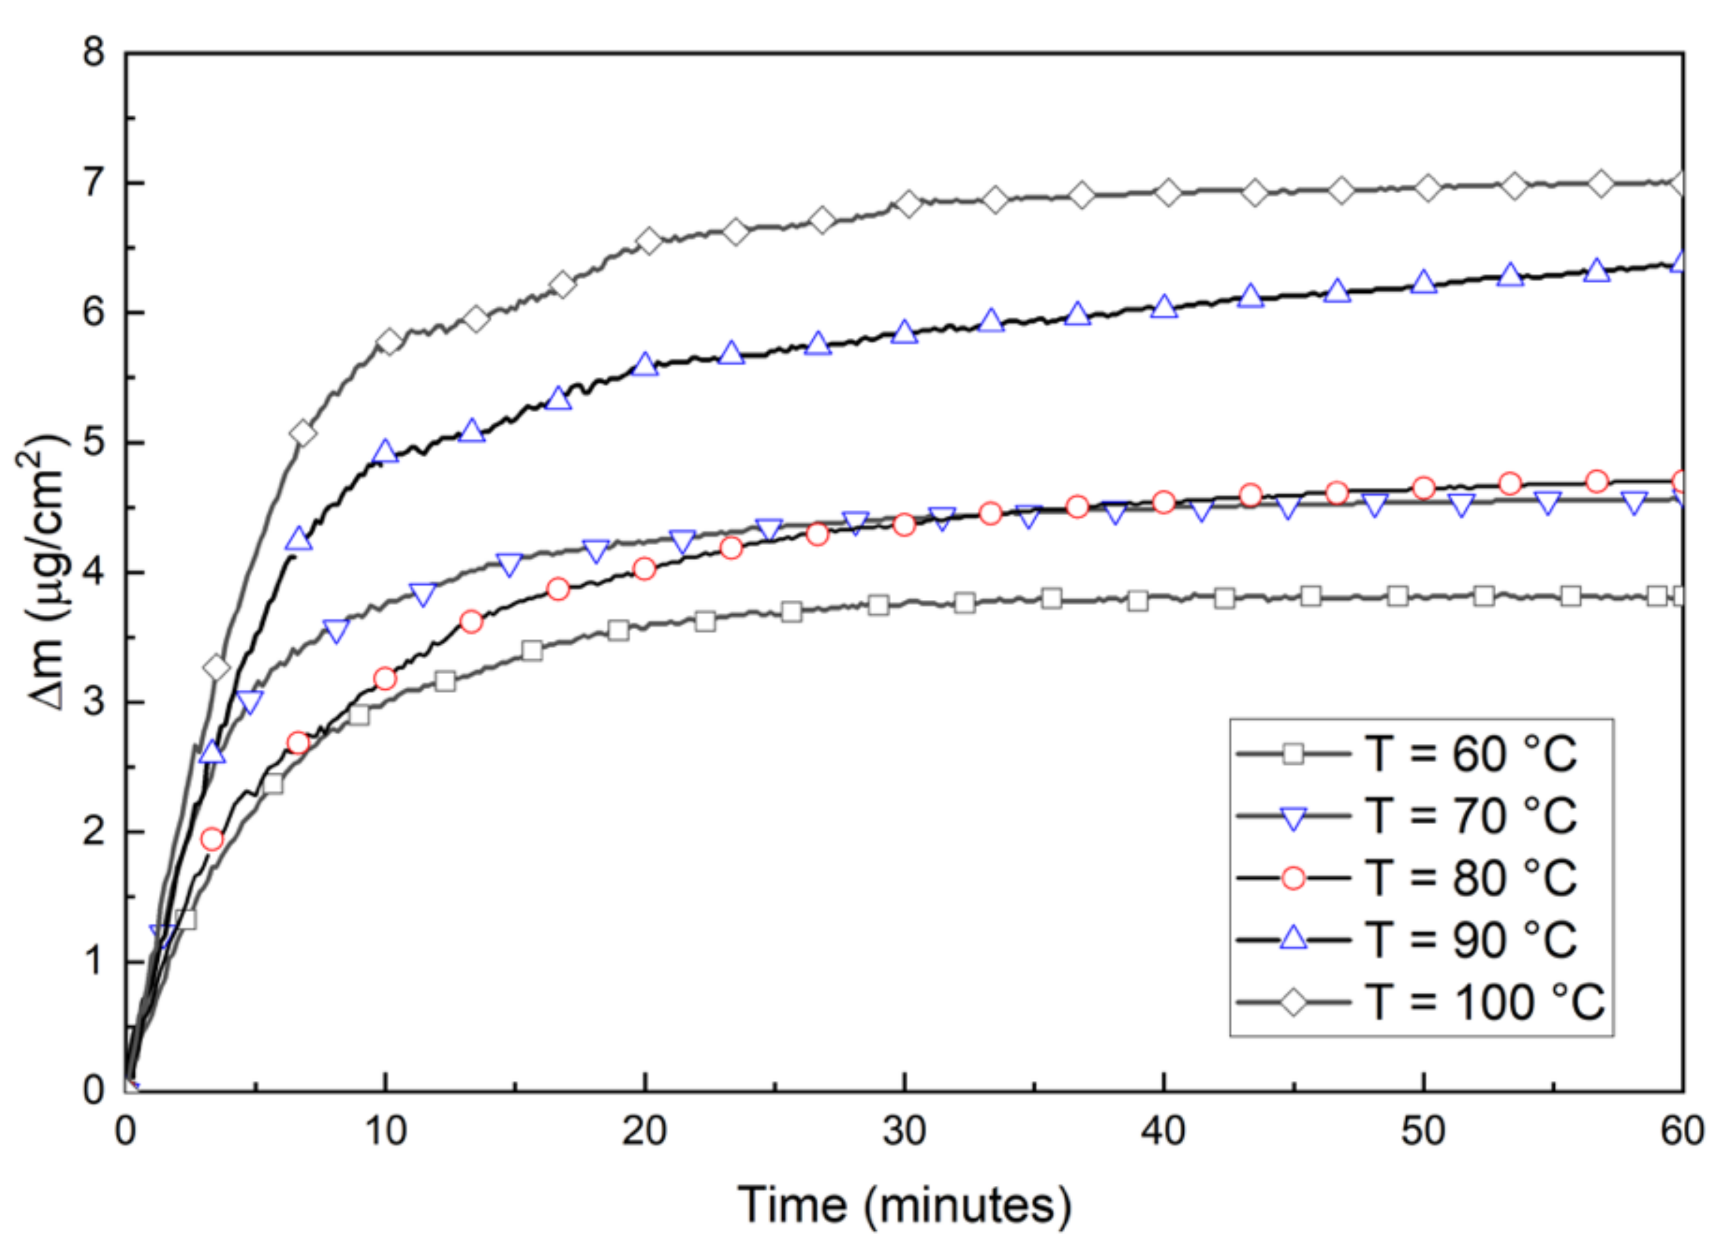
\includegraphics[width=0.5\textwidth]{img/21/Stud1.png}
    \label{fig:stud_1}
    \caption{Auszzug aus einer Studie, die die Massenänderung $\Delta m$ einer Kupferfläche auf einem Quarzkristall (QCM) pro Minute zeigt.}
\end{figure}
\begin{figure}[h!]
    \centering
    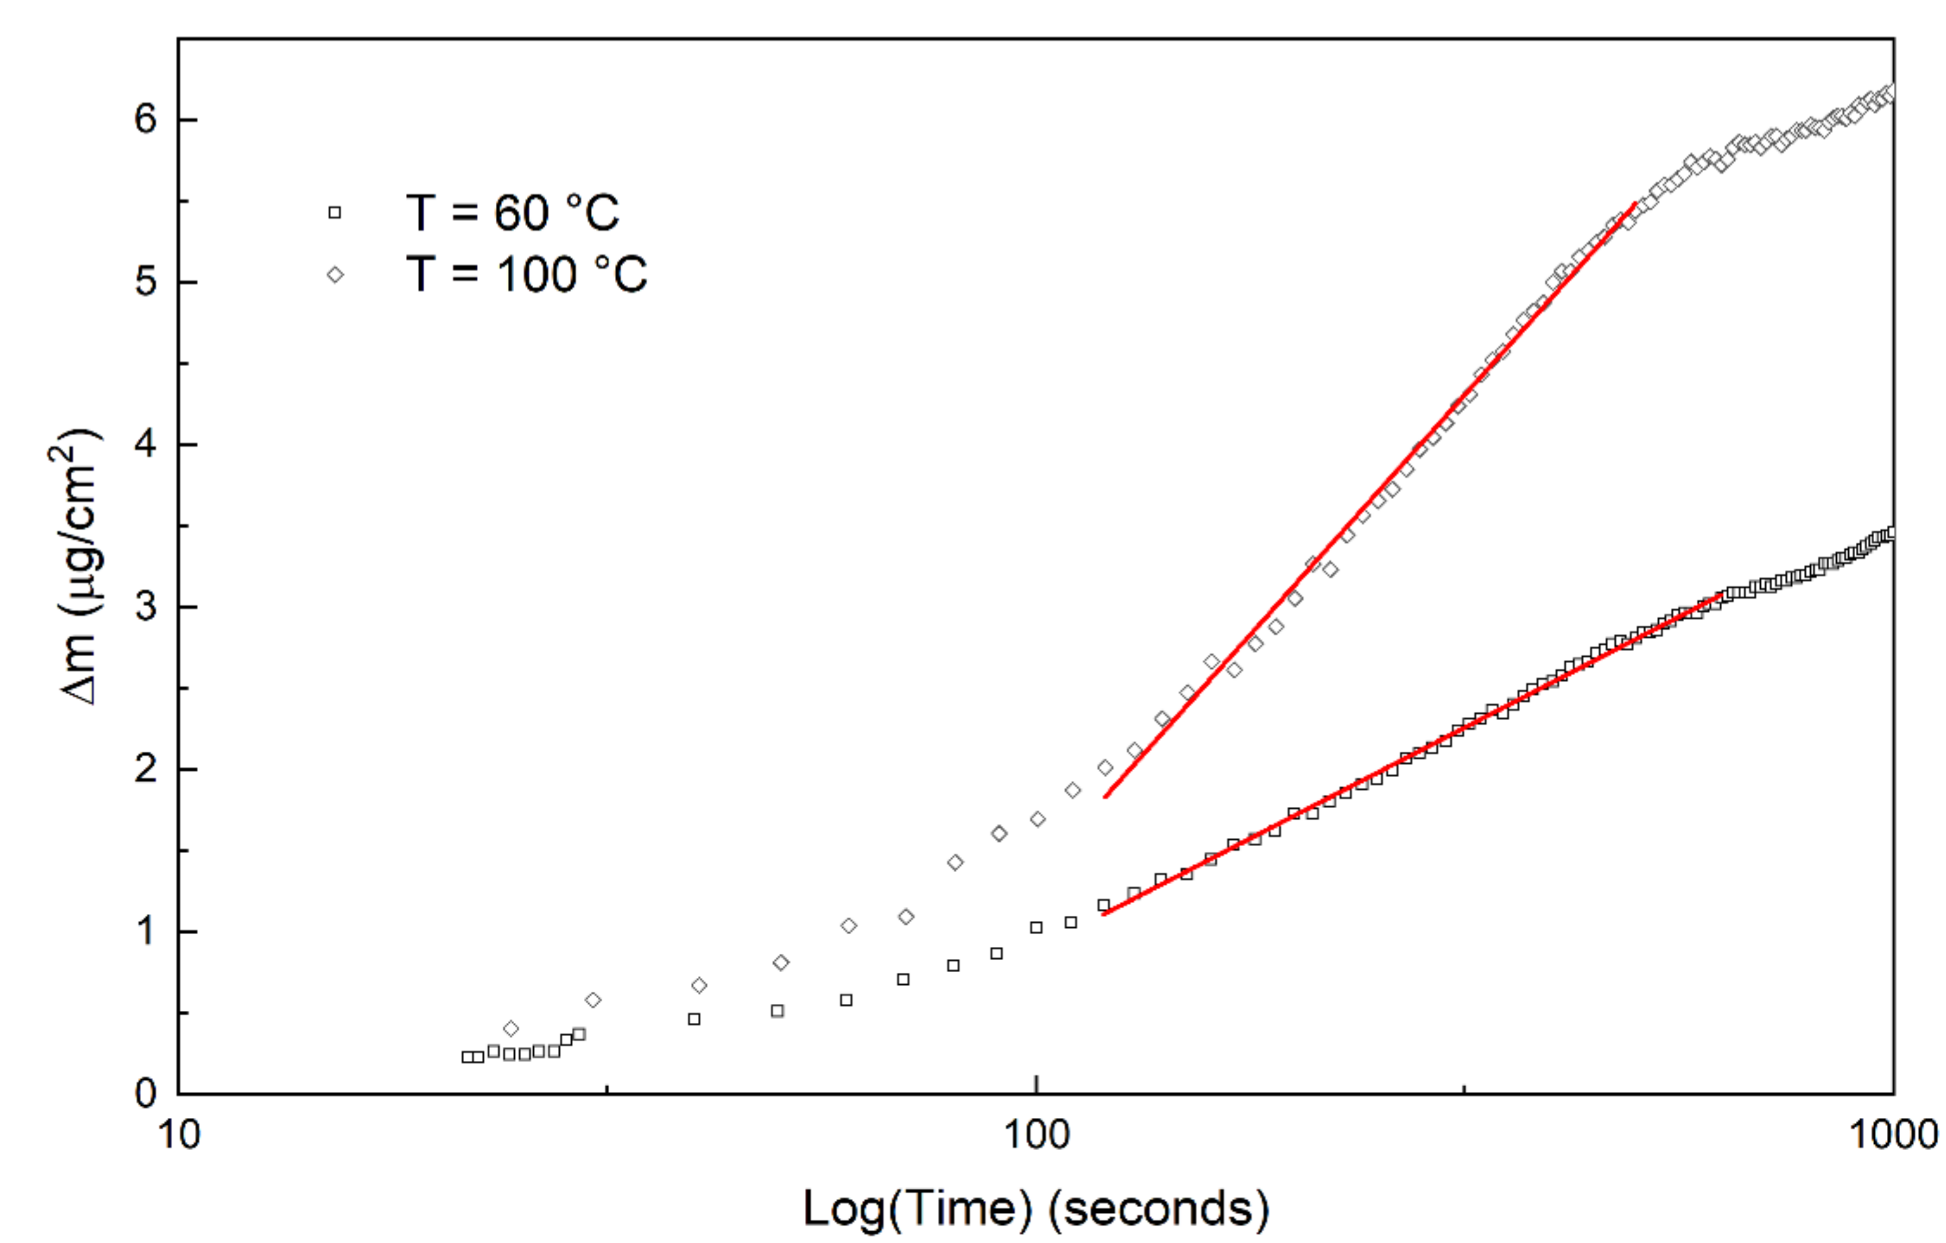
\includegraphics[width=0.5\textwidth]{img/21/Stud2.png}
    \label{fig:stud_2}
    \caption{Auszzug aus einer Studie, die die Massenänderung $\Delta m$ einer Kupferfläche auf einem Quarzkristall (QCM) pro Sekunde zeigt. Der Graph ist logarithmisch skaliert.}
\end{figure}

Für die \hyperref[fig:stud_2]{Abbildung (\ref*{fig:stud_2})} wurde die >>logarithmic rate constant<< berechnet. In der Studie steht die Gleichugn:
\begin{equation}
    \Delta m = k_{\log} \cdot \log(t) + C_{\log}.
    \label{eq:stud_log}
\end{equation}

Wobei \(\Delta m \) die Zunahme des Gewichts \([\mu\text{g cm}^{-2}]\),  
\( k_{\log} \) die logarithmische Geschwindigkeitskonstante \([\mu\text{g cm}^{-2} \log(\text{s}^{-1})]\),  
\( t \) die Zeit \([\text{s}]\) und  
\( C_{\log} \) \([\mu\text{g cm}^{-2}]\) das Gewicht des Oxids zu Beginn der logarithmischen Wachstumsperiode.

Dieser logarithmische Zusammenhang gilt nach den Autoren für rund um $20-25$ Minuten. Dannach stelle sich ein linearer anstig ein. Diesen können wir jedoch ignorieren, da wir diese Zeit nicht beobachten.
Dies ist in der \hyperref[fig:stud_2]{Abbildung (\ref*{fig:stud_2})} nicht exakt so zu entnehm.

Wir kommen in der \hyperref[ch:auswertung]{Auswertung} darauf zurück.